\documentclass[10pt, letterpaper, titlepage]{article} % Set font here.
% Use 'article' for simple documents; use 'report' for larger documents with chapters;
% use 'book' for even larger documents with parts.
\usepackage[utf8]{inputenc}
\usepackage{geometry}
\usepackage{color,graphicx,overpic} 
\usepackage{fancyhdr} % header/footer stuff
\usepackage{amsmath,amsthm,amsfonts,amssymb}
\usepackage{mathtools} % more math stuff
\usepackage{siunitx} % for SI units, ex. $3.5 ~ \si{kg.s^{-2}}$
\usepackage{hyperref} % for hyperlinks
\usepackage{apple_emoji}
\usepackage{multicol}
\usepackage{array}
\usepackage{float}
\usepackage{blindtext}
\usepackage{longtable}
\usepackage{scrextend}
\usepackage[font=small,labelfont=bf]{caption}
\usepackage[framemethod=tikz]{mdframed}
\usepackage{calc}
\usepackage{titlesec}
\usepackage{listings}
\usepackage[normalem]{ulem}

\usepackage{listings}
\usepackage{xcolor}

\DeclareMathOperator{\di}{d\!} % derivative operator symbol, ex. $\int f(x) \di x$
\newcommand{\Eval}[3]{\left.#1\right\rvert_{#2}^{#3}} % evaluation bar (ex. evaluating integral or $\Eval{F(x)}{0}{2}$)
\newcommand*\B{
\includegraphics[height=1.5em,valign=B,raise=-0.2em]{BigB.png}}
\newcommand*\fire{
\includegraphics[height=1.5em,valign=B,raise=-0.2em]{Fire.png}}

\definecolor{comment}{RGB}{140, 140, 140}
\definecolor{text}{RGB}{204, 204, 204}
\definecolor{string}{rgb}{0.58,0,0}
\definecolor{backcolour}{RGB}{27, 30, 39}
\definecolor{variable}{RGB}{244, 63, 78}

\lstdefinestyle{mystyle}{
    backgroundcolor=\color{backcolour},   
    commentstyle=\color{comment},
    keywordstyle=\color{variable},
    numberstyle=\tiny\color{text},
    stringstyle=\color{string},
    basicstyle=\ttfamily\footnotesize\color{text},
    breakatwhitespace=false,         
    breaklines=true,                 
    captionpos=b,                    
    keepspaces=true,                 
    numbers=left,                    
    numbersep=-10pt,                  
    showspaces=false,                
    showstringspaces=false,
    showtabs=false,                  
    tabsize=4
}

\lstdefinelanguage
   [x64]{Assembler}     % add a "x64" dialect of Assembler
   {morekeywords={	
   }} % etc.
   
\lstdefinelanguage[Motorola68k]{Assembler}{%
	morekeywords={	a0, a1, a2, a3, a4, a5, a6, a7, %
   					d0, d1, d2, d3, d4, d5, d6, d7, %
				   	ABCD,ADD,%
					ADDA,ADDI,ADDQ,ADDX,AND,ANDI,ASL,ASR,BCC,BLS,BCS,BLT,BEQ,BMI,BF,BNE,%
					BGE,BPL,BGT,BT,BHI,BVC,BLE,BVS,BCHG,BCLR,BRA,BSET,BSR,BTST,CHK,CLR,%
					CMP,CMPA,CMPI,CMPM,DBCC,DBLS,DBCS,DBLT,DBEQ,DBMI,DBF,DBNE,DBGE,DBPL,%
					DBGT,DBT,DBHI,DBVC,DBLE,DBVS,DIVS,DIVU,EOR,EORI,EXG,EXT,ILLEGAL,JMP,%
					JSR,LEA,LINK,LSL,LSR,MOVE,MOVEA,MOVEM,MOVEP,MOVEQ,MULS,MULU,NBCD,NEG,%
					NEGX,NOP,NOT,OR,ORI,PEA,RESET,ROL,ROR,ROXL,ROXR,RTE,RTR,RTS,SBCD,%
					SCC,SLS,SCS,SLT,SEQ,SMI,SF,SNE,SGE,SPL,SGT,ST,SHI,SVC,SLE,SVS,STOP,%
					SUB,SUBA,SUBI,SUBQ,SUBX,SWAP,TAS,TRAP,TRAPV,TST,UNLK},%
					sensitive=false,%
					morecomment=[l]*,%
					morecomment=[l] }[keywords,comments,strings]

\lstset{language=[Motorola68k]Assembler}
\lstset{style=mystyle}

\definecolor{mycolor}{rgb}{0, 0, 0}
  

\geometry{top=2.7cm,left=1.8cm,right=1.8cm,bottom=2.7cm}
\setlength{\headheight}{17pt}
\renewcommand{\baselinestretch}{1.5} 
\setlength{\parskip}{0.3cm}
\setlength{\parindent}{0.6cm}
\titlespacing\section{0pt}{12pt plus 4pt minus 2pt}{0pt plus 2pt minus 2pt}

\newcommand{\barrows}{\textcolor{blue}{\Longrightarrow}\quad}
\newcommand{\barrow}{\quad\textcolor{blue}{\Longrightarrow}\quad}  
\newcommand{\sumi}[1][1]{ \sum_{n={#1}}^{\infty} }
\newcommand{\limi}[1][n]{ \lim_{{#1}\to\infty} }

\title{\textbf{\Huge{
\begin{center}
Hardware Interfacing \\ 😂😂😂 \\
\end{center}
}}}
\author{\B enjamin Kong | 1573684\\Lora Ma ||||| 1570935\\ \\ECE 212 Lab Section H11}

\pagestyle{fancy}
\fancyhf{}
\rhead{\B enjamin Kong \& Lora Ma}
\lhead{\textit{Hardware Interfacing 😂😂😂}}
\rfoot{Page \thepage}

\begin{document} 
\pagenumbering{gobble} 
\maketitle 
\thispagestyle{empty}
\tableofcontents 
\newpage
\pagenumbering{arabic}

\section{Discussion}

Due to the COVID-19 pandemic, we were unable to physically complete the hardware component of the lab. As a result, the majority of this lab report will be focused on how the software component (i.e., the assembly language programming) works with the hardware component of the lab. We will discuss various details regarding the hardware and software working together. We will also outline the different parts of the lab and what purposes they each fulfill.

The purpose of this lab was to gain experience using the Netburner board to interface with hardware. We were to use the Netburner board connected with a bufferboard to interface with the GMC2288C 8x8 LED array. Furthermore, we were to use two 3x8 74LS138 decoders, 8 $\SI{1}{k\Omega}$ resistors, and two hex-input 74LS04 inverters. 

The Netburner board uses a 10-pin ribbon cable to interface with the bufferboard. This 10-pin ribbon cable maps pins 37 to 43 of the Netburner to the bufferboard. The bufferboard is then connected to various parts of the breadboard, which contains the LED array. 

We now discuss the software component of the lab, which we were able to complete (despite not being able to test it with the hardware). There were three parts to the lab:
\begin{enumerate}
\item WelcomePrompt,
\item Convert, and
\item LedSub.
\end{enumerate}
In the first part of the lab (WelcomePrompt), we wrote a subroutine that prompts the user to enter a single keystroke from the keyboard. We first display a welcome message, then prompt the user for a string. When the user inputs something, we check that the character is valid. An invalid input results in re-prompting the user for input. We then place the character (stored in ASCII format) onto the stack, at which point we pass it on to the Convert subroutine (which is the next part of the lab).

For the second part of the lab (Convert), we take the keystroke from the stack and pass out the pattern address through the stack. This pattern is stored as 2 longwords (2 bytes), and we use the subrountine called convert1 (provided to us) to get the pattern. We then move on to the LedSub subroutine (the last part of the lab).

For the third part of the lab (LedSub), we take the pattern address passed from the stack to display the pattern onto the 8x8 LED array. We then loop through the array and check if each LED should be switched on or off. After we iterate through the subroutine, we do a 300 unit delay such that information the LED array displays is visible.

We have included UML diagrams for each respective part of the lab in the appendix, along with our code.

\section{Question}

\textit{Why were the two 74LS138 decoders used in the circuit instead of directly connecting the pins to the
array? Discuss how removing the decoders would affect the function of the LED array in the context of this lab.}

If we didn't use the two decoders, we would require a wider ribbon cable (a 16 pin one) from the Netburner board to the bufferboard. This is because each row/column in the LED array has 8 positions; hence, we need 3 bits to access any position in a row/column. Hence without the decoders, we'd need 6 extra input pins. We would have to select LEDs in the LED array directly from the microprocessor; hence, we would have to modify the subroutines in LedSub to select pins directly.

\newpage

\section{Appendix}

\subsection{Part A UML Diagram}
\begin{figure}[H]
   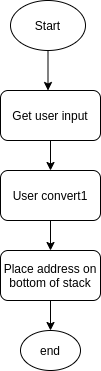
\includegraphics[width=0.12\textwidth]{UML1.png}
   \centering  
   \caption{UML diagram for part A.} 
   \label{figure:1}
\end{figure}

\subsection{Part B UML Diagram}
\begin{figure}[H]
   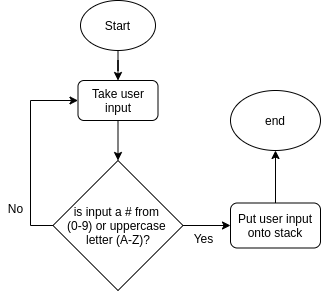
\includegraphics[width=0.4\textwidth]{UML2.png}
   \centering  
   \caption{UML diagram for part B.} 
   \label{figure:2}
\end{figure}

\subsection{Part C UML Diagram}
\begin{figure}[H]
   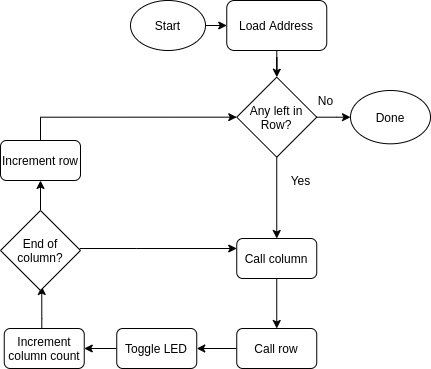
\includegraphics[width=0.5\textwidth]{UML3.png}
   \centering  
   \caption{UML diagram for part C.} 
   \label{figure:3}
\end{figure}

\subsection{Part A Assembler Code}
\begin{lstlisting}
	WelcomePrompt:
	/*Write your program here******************************************/
	
	/* Backup registers */
	LEA -40(%sp), %sp
	MOVEM.L %D2-%D5/%A2-%A5, (%sp)
	
	/* Display Welcome message */
	pea Welcome
	jsr iprintf
	adda.l #4, %sp
	jsr cr
	
	/* Prompt for string */
	PEA Ask
	JSR iprintf
	ADDA.L #4, %sp
	JSR cr
	BRA GetChar
	
	Invalid:
	  PEA InvalidInput
	  JSR iprintf
	  ADDA.L #4, %sp
	  JSR cr
	
	GetChar:
	  JSR getchr
	  CMPI.L #48, %D0
	  BLT Invalid
	  CMPI.L #57, %D0
	  BGT Check
	
	Check:
	  CMPI.L  #65, %D0
	  BLT Invalid
	  CMPI.L  #90, %D0
	  BGT Invalid
	
	/* Move ASCII Keystroke to location */
	MOVE.L %d0, 44(%sp)
	
	
	/* Restore registers */
	MOVEM.L (%sp), %D2-%D5/%A2-%A5
	LEA     40(%sp), %sp
	
	rts
	/*End of Subroutine **************************************************/
	.data
	/*All Strings placed here **************************************************/
	
	Welcome:
	.string "Welcome to Wing's LED Display"
	
	Ask:
	.string "Please enter an UpperCase letter or Number from the keyboard"
	
	InvalidInput
	.string "Invalid entry, please enter proper keystroke from keyboard"
	
	/*End of Strings **************************************************/
	/******************************************************/	
\end{lstlisting}

\subsection{Part B Assembler Code}
\begin{lstlisting}
	convert:
	/*Write your program here******************************************/
	
	/* Backup registers */
	LEA -40(%sp), %sp
	MOVEM.L %D2-%D5/%A2-%A5, (%sp)
	
	MOVE.L 44(%sp), -(%sp)
	JSR convert1
	MOVE.L (%sp)+, 44(%sp)
	
	/* Restore registers */
	MOVEM.L (%sp), %D2-%D5/%A2-%A5
	LEA 40(%sp), %sp
	
	rts 
	
	/*End of Subroutine **************************************************/ 
	.data
	/*All Strings placed here **************************************************/
	
	
	/*End of Strings **************************************************/
\end{lstlisting}

\subsection{Part C Assembler Code}

\begin{lstlisting}
	LedSub:
	/*Write your program here******************************************/
	LEA -40(%A7),%A7
	MOVEM.L %D2-%D7/%A2-%A5,(%A7)
	
	MOVEA.L 44(%A7), %A2 /* Load address*/
	CLR.L %D3
	CLR.L %D2
	
	LoopRow:
	CMP.L #8, %D2 /* Check if loop is done */
	BGE End
	MOVE.B (%A2, %D2*1), %D4 /* Load row */
	
	LoopColumn:
	MOVE.L %D3, -(%sp)
	JSR Column
	LEA 4(%sp), (%sp) /* Clean up stack */
	
	MOVE.L %D2, -(%sp) /* Load row number in to stack */
	JSR Row /* Call row subroutine */
	LEA 4(%sp), (%sp) /* Clean up stack */
	MOVE.L %D3, %D5
	ADD.L #-7, %D5
	BTST.B %D5, %D4
	BEQ TurnOff
	JSR TurnOnLed /* Turn on if 1 */
	BRA Loop
	
	TurnOff:
	JSR TurnOffLed /* Turn off if 0 */
	BRA PostLoop
	
	Loop:
	ADD.L #1, %D3 /* Increment column */
	CMP.L #8, %D3
	BLT LoopColumn
	CLR.L %D3
	ADD.L #1, %D2 /* Increment row */
	BRA LoopRow /* return to row loop */
	
	End:
	MOVE.L #300, -(%sp)
	JSR Delay /* Call delay subroutine */
	LEA 4(%sp), (%sp) /* Clean up stack */
	
	MOVEM.L (%A7), %D2-%D7/A2-%A5
	LEA 40(%A7),%A7
	
	
	rts
	/*End of Subroutine **************************************************/
	.data
	/*All Strings placed here **************************************************/
	
	
	
	/*End of Strings **************************************************/
	/******************************************************/
\end{lstlisting}

\end{document}
